\documentclass[aspectratio=169]{beamer}
\usepackage{fontspec}
\usepackage{graphicx}
\usepackage{tikz}
\usepackage{xcolor}
\usetikzlibrary{calc}  

% Define custom color
\definecolor{vyperblack}{HTML}{180C25}
\definecolor{vyperviolet}{HTML}{9F4CF2}
\definecolor{bubblecolor}{HTML}{DDCEAF}
\definecolor{numbertextcolor}{HTML}{FDFCFB}


% Set Inconsolata as the main font and for all text elements
\setmainfont{Inconsolata}[
Path = /usr/share/fonts/TTF/,
Extension = .ttf,
UprightFont = *-Regular,
BoldFont = *-Bold,
ItalicFont = *-Regular,
BoldItalicFont = *-Bold
]
\setsansfont{Inconsolata}[
Path = /usr/share/fonts/TTF/,
Extension = .ttf,
UprightFont = *-Regular,
BoldFont = *-Bold,
ItalicFont = *-Regular,
BoldItalicFont = *-Bold
]

% Set SemiExpanded Bold for titles
\newfontfamily\titlefont{Inconsolata}[
Path = /usr/share/fonts/TTF/,
Extension = .ttf,
UprightFont = *_SemiExpanded-Bold,
BoldFont = *_SemiExpanded-Bold,
ItalicFont = *_SemiExpanded-Bold,
BoldItalicFont = *_SemiExpanded-Bold
]

% Set theme
\usetheme{default}
\usecolortheme{default}

% Remove navigation symbols
\setbeamertemplate{navigation symbols}{}

% Custom background
\setbeamertemplate{background}{
	
\includegraphics[width=\paperwidth,height=\paperheight]{supergraphic.png}
}

% Custom title page
\setbeamertemplate{title page}{
	\begin{tikzpicture}[remember picture,overlay]
		\node[anchor=north west,yshift=-20pt,xshift=20pt] at (current page.north west) {
			
\includegraphics[width=0.25\textwidth]{vyper-logo-landscape-color-pos.pdf}
		};
		\node[anchor=north west,yshift=-20pt,xshift=20pt] at (current page.north west) {
			\parbox{0.95\textwidth}{\vspace{3.25cm}\raggedright\fontsize{40}{48}\selectfont\titlefont\textcolor{vyperblack}{\textbf{\inserttitle}}}
		};
	\end{tikzpicture}
}

% Custom frame title
\setbeamertemplate{frametitle}{
	\begin{tikzpicture}[remember picture,overlay]
		\node[anchor=north west,yshift=-10pt,xshift=10pt] at (current page.north west) {
			
\includegraphics[width=0.04\textwidth]{VYPER_SYMBOL_COLOR.png}
		};
		\node[anchor=north west,yshift=-10pt,xshift=0.11\textwidth] at (current page.north west) {
			\parbox{0.94\textwidth}{\raggedright\fontsize{24}{26}\titlefont\textcolor{vyperblack}{\textbf{\insertframetitle}}}
		};
	\end{tikzpicture}
}

% Set all text to vyperblack
\setbeamercolor{normal text}{fg=vyperblack}
\setbeamercolor{frametitle}{fg=vyperblack}
\setbeamercolor{title}{fg=vyperblack}

\title{Vyper Roadmap \\ Growth \& Funding}

\begin{document}
	
	% Title slide
	\begin{frame}[plain]
		\titlepage
	\end{frame}
	
	% Second slide - KPI
	\begin{frame}
		\frametitle{Vyper at a Glance}
		\begin{columns}[T,totalwidth=\textwidth]
			\begin{column}{0.5\textwidth}
				\begin{center}
					\textcolor{vyperviolet}{\fontsize{40}{48}\selectfont\textbf{\$4.1b}}
					\vspace{0.5em}
					
					\small Total Value Locked\\in Vyper Contracts
				\end{center}
			\end{column}
			\begin{column}{0.5\textwidth}
				\begin{center}
					\textcolor{vyperviolet}{\fontsize{40}{48}\selectfont\textbf{2\textsuperscript{nd}}}
					\vspace{0.5em}
					
					\small Most popular EVM language
				\end{center}
			\end{column}
		\end{columns}
		
		\vspace{1em}
		
		\begin{columns}[T,totalwidth=\textwidth]
			\begin{column}{0.5\textwidth}
				\begin{center}
					\textcolor{vyperviolet}{\fontsize{40}{48}\selectfont\textbf{10}}
					\vspace{0.5em}
					
					\small New Vyper contracts\\deployed every day
				\end{center}
			\end{column}
			\begin{column}{0.5\textwidth}
				\begin{center}
					\textcolor{vyperviolet}{\fontsize{40}{48}\selectfont\textbf{100+}}
					\vspace{0.5em}
					
					\small Contributors on Github
				\end{center}
			\end{column}
		\end{columns}
	\end{frame}
	
	% Third Slide - Protocols using Vyper
	\begin{frame}
		\frametitle{They use Vyper}
		\centering
		\begin{tikzpicture}[remember picture,overlay]
			% Top row
			\foreach \x/\name in {0/Curve, 1/Frax, 2/Lido, 3/{Perpetual Protocol}}
			{
				\node[anchor=north] at ($(current page.north)+(-0.375\paperwidth+0.25\paperwidth*\x,-0.18\paperheight)$) {
					\includegraphics[width=0.12\paperwidth]{users/\name.png}
				};
				\node[anchor=north, text width=0.18\paperwidth, align=center] at ($(current page.north)+(-0.375\paperwidth+0.25\paperwidth*\x,-0.43\paperheight)$) {
					\large\name
				};
			}
			
			% Bottom row
			\foreach \x/\name in {0/Velodrome, 1/Yearn, 2/{Sorella Labs}}
			{
				\node[anchor=north] at ($(current page.north)+(-0.25\paperwidth+0.25\paperwidth*\x,-0.56\paperheight)$) {
					\includegraphics[width=0.12\paperwidth]{users/\name.png}
				};
				\node[anchor=north, text width=0.18\paperwidth, align=center] at ($(current page.north)+(-0.25\paperwidth+0.25\paperwidth*\x,-0.86\paperheight)$) {
					\large\name
				};
			}
		\end{tikzpicture}
	\end{frame}
	
	% Fourth Slide - Vision
	\begin{frame}
		\frametitle{Vision}
		\setbeamercolor{itemize item}{fg=vyperviolet}
		\setbeamercolor{itemize subitem}{fg=vyperviolet}
		\setbeamercolor{itemize subsubitem}{fg=vyperviolet}
		\begin{itemize}
			\item Despite a growing user base and adoption by major DeFi protocols, \textbf{Vyper contracts account for less than 1\% of all new contract deployments}.
			\vspace{1em}
			\item We want to bring this number to \textbf{50\% by 2028.}
			\vspace{1em}
			\item This is the only path to achieve language diversity on Ethereum.
		\end{itemize}
	\end{frame}
	
	% Fifth Slide - User Acquisition
	\begin{frame}
		\frametitle{User Acquisition Pathways}
		\begin{tikzpicture}[remember picture,overlay]
			\foreach \x/\title/\itemA/\itemB [count=\i] in {
				0/{Converting Developers}/{Experienced Solidity developers switching to Vyper for their next project}/{Protocols written in Solidity adding new contracts written in Vyper},
				1/{Onboarding Developers}/{Bringing experienced web2 developers to web3}/{Becoming the language of choice for all beginner web3 developers}
			} {
				\node[anchor=north west, 
				fill=bubblecolor!70, 
				opacity=0.5,
				rounded corners, 
				text width=0.85\paperwidth,
				inner sep=15pt,
				minimum height=8em] 
				at ($(current page.north west)+(0.03\paperwidth,-0.22\paperheight-0.32\paperheight*\x)$) 
				(bubble\i) {};
				
				\node[circle, 
				fill=vyperviolet, 
				text=numbertextcolor, 
				font=\bfseries, 
				minimum size=1.5em] 
				at ($(bubble\i.north west)+(0.5em,-0.5em)$) 
				{\i};
				
				\node[anchor=north west, 
				font=\bfseries, 
				text width=0.8\paperwidth] 
				at ($(bubble\i.north west)+(2em,-0.5em)$) 
				{\title};
				
				\node[anchor=north west, 
				font=\footnotesize, 
				text width=0.8\paperwidth] 
				at ($(bubble\i.north west)+(1em,-2.5em)$) 
				{$\bullet$ \itemA\\[0.5em]$\bullet$ \itemB};
			}
		\end{tikzpicture}
	\end{frame}
	
	% Revenue Slide
	\begin{frame}
		\frametitle{Funding Sources (Grants)}
		\begin{columns}[T,totalwidth=\textwidth]
			\begin{column}{0.4\textwidth}
				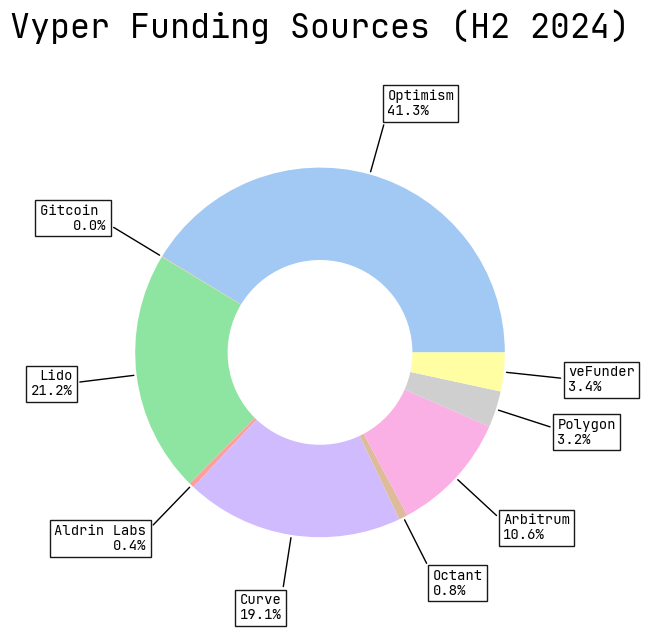
\includegraphics[width=\columnwidth]{charts/revenue.png}
			\end{column}
			\begin{column}{0.55\textwidth}
				\setbeamercolor{itemize item}{fg=vyperviolet}
				\setbeamercolor{itemize subitem}{fg=vyperviolet}
				\setbeamercolor{itemize subsubitem}{fg=vyperviolet}
				\begin{itemize}
					\item Sustainable funding is diversified funding
					\vspace{0.5em}
					\item We are working to establish relationships and trust with funders to ensure more consistent and sizeable funding in the future
					\vspace{0.5em}
					\item Protocols using the language have been major funders. Increasing Vyper adoption helps ensure sustainable funding
				\end{itemize}
			\end{column}
		\end{columns}
	\end{frame}
	
	% Grant Funding Slide
	\begin{frame}
		\frametitle{Targeted Grants}
		\begin{tikzpicture}[remember picture,overlay]
			\foreach \x/\y/\title/\items [count=\i] in {
				0/0/{Public Goods Funding}/{Optimism RPGF, Octant, Gitcoin, EF, ENS, VeFunder,  Giveth, Dev Tooling Guild},
				1/0/{L2 Ecosystem Grants}/{Arbitrum, Optimism, Polygon, Scroll, Sonic Labs, Manta, Taiko},
				0/1/{Protocols (Rev Share/Grants) }/{Curve, Lido, Yearn, Frax, Aldrin Labs, Drips},
				1/1/{Non-web3 Grants}/{Academic Grants for R\&D, Python Foundation},
				0.5/2/{Direct Donations}/{Benevity, Llamas NFT, Developers, KOLs}
			} {
				\node[anchor=north west, 
				fill=bubblecolor!70, 
				opacity=0.5,
				rounded corners, 
				text width=0.4\paperwidth,
				inner sep=10pt,
				minimum height=5em] 
				at ($(current page.north west)+(0.03\paperwidth+0.49\paperwidth*\x,-0.22\paperheight-0.25\paperheight*\y)$) 
				(bubble\i) {};
				
				\node[circle, 
				fill=vyperviolet, 
				text=numbertextcolor, 
				font=\bfseries, 
				minimum size=1.5em] 
				at ($(bubble\i.north west)+(0.5em,-0.5em)$) 
				{\i};
				
				\node[anchor=north west, 
				font=\bfseries, 
				text width=0.4\paperwidth] 
				at ($(bubble\i.north west)+(2em,-0.5em)$) 
				{\title};
				
				\node[anchor=north west, 
				font=\footnotesize, 
				text width=0.4\paperwidth] 
				at ($(bubble\i.north west)+(0.5em,-2.5em)$) 
				{\items};
			}
		\end{tikzpicture}
	\end{frame}
	
	\begin{frame}
		\frametitle{Funding Sources (Commercial)}
		\begin{tikzpicture}[remember picture,overlay]
			\foreach \x/\y/\title/\items [count=\i] in {
				0/0/{Consulting}/{Code reviews, personalized assistance, advice on best practices, introductions to builders \& auditors},
				1/0/{Tooling Licensing}/{Introduce a freemium model for current (Titanoboa) or future (shadow events, debugger) tooling developed by the team},
				0/1/{Paid Partnerships}/{Protocols or L2s give funding in exchange for accelerated support of their chain and visibility (in docs, site \& socials)},
				1/1/{Token Allocations}/{Negotiate allocations from new protocols building with Vyper in exchange for assistance and/or promotion}
			} {
				\node[anchor=north west, 
				fill=bubblecolor!70, 
				opacity=0.5,
				rounded corners, 
				text width=0.4\paperwidth,
				inner sep=10pt,
				minimum height=7em] 
				at ($(current page.north west)+(0.03\paperwidth+0.49\paperwidth*\x,-0.22\paperheight-0.35\paperheight*\y)$) 
				(bubble\i) {};
				
				\node[circle, 
				fill=vyperviolet, 
				text=numbertextcolor, 
				font=\bfseries, 
				minimum size=1.5em] 
				at ($(bubble\i.north west)+(0.5em,-0.5em)$) 
				{\i};
				
				\node[anchor=north west, 
				font=\bfseries, 
				text width=0.4\paperwidth] 
				at ($(bubble\i.north west)+(2em,-0.5em)$) 
				{\title};
				
				\node[anchor=north west, 
				font=\footnotesize, 
				text width=0.4\paperwidth] 
				at ($(bubble\i.north west)+(0.5em,-2.5em)$) 
				{\items};
			}
		\end{tikzpicture}
	\end{frame}
\end{document}